\section{Results}
\label{sec:results}

\subsection{Curve reproduction and shape}
\label{sec:curvefit}

The constrained solve reproduces all six monthly averages to a maximum absolute
error of $3.6\times10^{-12}$ \TRY{} (Figure~\ref{fig:monthlyfit}), which
establishes only that the constraint set is satisfied, for the reason given in
Section~\ref{sec:curve}.

\begin{figure}[htbp]
\centering
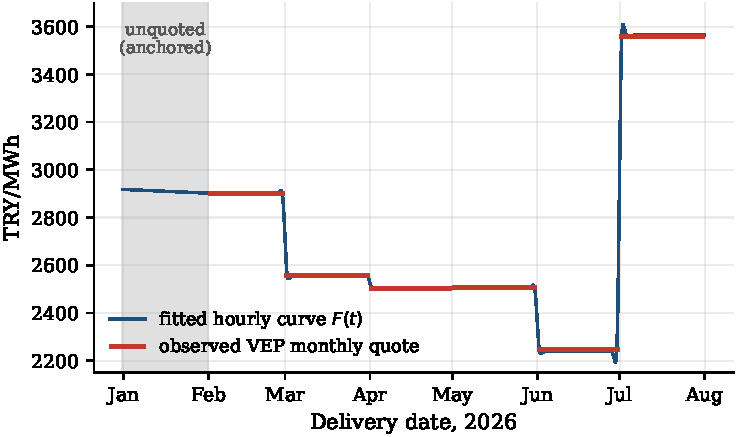
\includegraphics[width=\textwidth]{figures/fwd_curve.pdf}
\caption{Fitted hourly forward curve against the observed monthly baseload
quotes. Shading marks the unquoted January window.}
\label{fig:monthlyfit}
\end{figure}

The shape of the curve is more informative than the fit. Hourly increments have
a mean absolute size of $0.45$ \TRY, and the three largest increments over the
whole horizon sit at month boundaries where the quote strip itself steps, the
largest being $+47.0$ \TRY{} at June--July. That step reflects the $58\%$ rise
between the June and July quotes and is therefore a property of the data rather
than an artefact of interpolation. Within the January window the largest
increment is $0.05$ \TRY, so the anchor joins the quoted region without a
discontinuity, and no oscillation of the kind unconstrained spline interpolation
can produce near sharp level changes is present.

\subsection{Baseline valuation and the option surface}
\label{sec:surface}

At the reference contract, a European call struck at $3{,}000$ \TRY{} expiring
$72$ hours after valuation, the model gives $F(T) = 2{,}916.16$ \TRY, terminal
residual standard deviation $532.26$ \TRY, and a value of $166.75$ \TRY{} by
finite differences against $169.18$ \TRY{} by simulation. The simulated
probability of a negative terminal price is zero at four decimal places, so the
additive specification, while unbounded below in principle, is not operating
near that boundary at the calibrated dispersion.

Table~\ref{tab:surface} reports the surface at three representative strikes,
and Figure~\ref{fig:surface} displays the grid as strike and maturity sections.
Sections are preferred to a perspective surface because exact values remain
readable.

\begin{table}[htbp]
\centering
\caption{Expiry-hour European option values from the production configuration.
All expiries fall inside the unquoted January window. All quantities in \TRY.}
\label{tab:surface}
\small
\begin{tabular}{rrrrrr}
\toprule
Maturity (h) & Strike & $F(T)$ & Call & Put & Residual SD \\
\midrule
\multirow{3}{*}{24}  & 2{,}000 & 2{,}917.24 & 927.11 & 10.87 & \multirow{3}{*}{524.08} \\
                     & 3{,}000 & 2{,}917.24 & 163.93 & 246.60 & \\
                     & 4{,}000 & 2{,}917.24 & 5.59 & 1{,}087.16 & \\
\midrule
\multirow{3}{*}{72}  & 2{,}000 & 2{,}916.16 & 924.70 & 11.55 & \multirow{3}{*}{532.26} \\
                     & 3{,}000 & 2{,}916.16 & 166.75 & 250.32 & \\
                     & 4{,}000 & 2{,}916.16 & 5.94 & 1{,}086.22 & \\
\midrule
\multirow{3}{*}{336} & 2{,}000 & 2{,}910.21 & 907.92 & 11.57 & \multirow{3}{*}{531.19} \\
                     & 3{,}000 & 2{,}910.21 & 161.84 & 250.27 & \\
                     & 4{,}000 & 2{,}910.21 & 5.66 & 1{,}078.86 & \\
\midrule
\multirow{3}{*}{720} & 2{,}000 & 2{,}901.51 & 883.95 & 11.60 & \multirow{3}{*}{529.61} \\
                     & 3{,}000 & 2{,}901.51 & 154.91 & 250.21 & \\
                     & 4{,}000 & 2{,}901.51 & 5.28 & 1{,}068.24 & \\
\bottomrule
\end{tabular}
\end{table}

\begin{figure}[htbp]
\centering
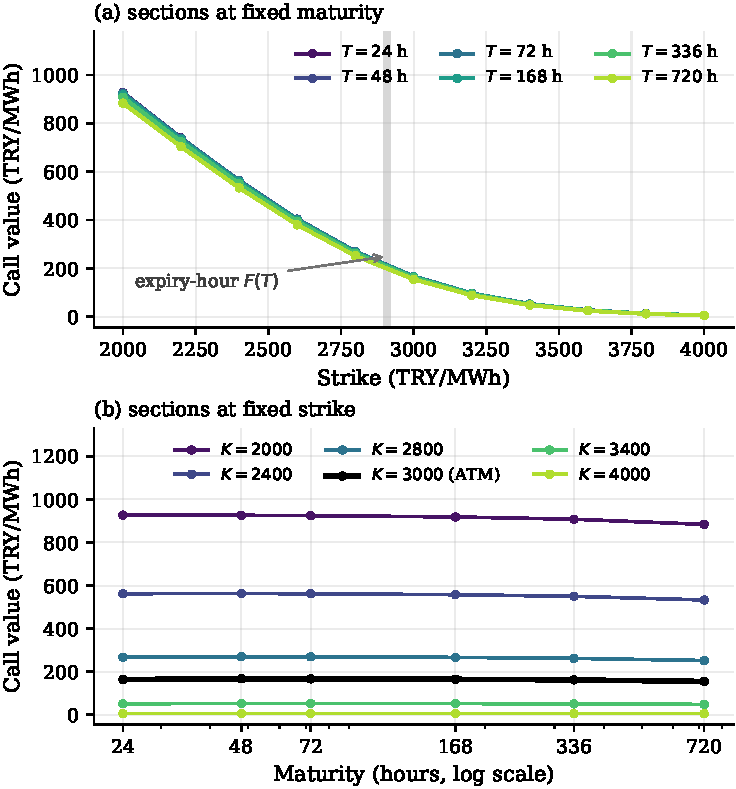
\includegraphics[width=\textwidth]{figures/option_surface.pdf}
\caption{Two sections through the option price surface. Panel (a) shows call
value against strike at each maturity, with shading marking the range of
expiry-hour forward levels; panel (b) shows call value against maturity at
representative strikes, the near-at-the-money strike emphasised.}
\label{fig:surface}
\end{figure}



One feature of the surface separates it from the term structure of a diffusive
model and follows directly from the mean-reverting residual: terminal dispersion
saturates rather than growing (Figure~\ref{fig:residualsd}). With a half-life of
$8.84$ hours the residual reaches its stationary distribution within roughly a
day, after which option value varies with maturity almost entirely through the
forward level and the discount factor rather than through accumulated
uncertainty. The mild decline in at-the-money value across the maturities in
Table~\ref{tab:surface} is therefore attributable to the downward slope of the
anchored January curve rather than to any reduction in volatility.

\begin{figure}[htbp]
\centering
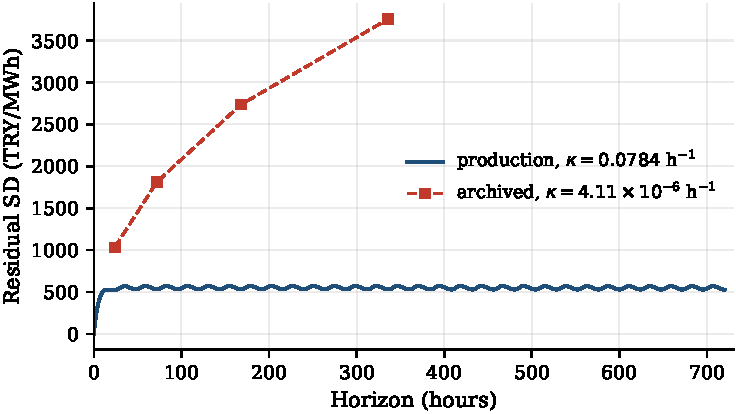
\includegraphics[width=\textwidth]{figures/residual_sd.pdf}
\caption{Terminal residual standard deviation against horizon, production
against archived specification.}
\label{fig:residualsd}
\end{figure}

\subsection{Sensitivity to unidentified inputs}
\label{sec:sensitivity}

Table~\ref{tab:sensitivity} collects controlled experiments in which a single
input is varied and everything else is held at production values. We order them
by the magnitude of the resulting price change, because that ordering is itself
the main result of this section.

\begin{table}[htbp]
\centering
\caption{Controlled sensitivity of the $72$-hour, $K=3{,}000$ call. Each row
varies one input; all others are held at production values. Baseline
$166.75$ \TRY.}
\label{tab:sensitivity}
\small
\setlength{\tabcolsep}{5pt}
\begin{tabular}{@{}llrr@{}}
\toprule
Input varied & Perturbation & Call (\TRY) & Change \\
\midrule
January anchor level & $-20\%$ & 17.80 & $-89.3\%$ \\
January anchor level & $-10\%$ & 65.75 & $-60.6\%$ \\
January anchor level & $+10\%$ & 326.05 & $+95.5\%$ \\
January anchor level & $+20\%$ & 528.96 & $+217.2\%$ \\
\midrule
Mean-reversion rate & archived near-unit-root value & 687.04 & $+312.0\%$ \\
\midrule
Residual demand path & $-2\sigma$ offset & 200.81 & $+20.4\%$ \\
Residual demand path & $+2\sigma$ offset & 107.97 & $-35.2\%$ \\
\midrule
Regime volatilities & alternative model estimate & 165.58 & $-0.70\%$ \\
Discount rate & $r=0.15$ & 167.09 & $+0.21\%$ \\
Discount rate & $r=0.60$ & 166.47 & $-0.16\%$ \\
Initial regime distribution & stationary rather than filtered & 166.75 & $+0.0003\%$ \\
Drift premium $a_1$ & plausible magnitudes & 166.75 & $<10^{-4}\%$ \\
\bottomrule
\end{tabular}
\end{table}

\paragraph{The anchor dominates everything else.}
\label{sec:anchorsens}
Shifting the January anchor level by $\pm20\%$, holding the curve shape rule
fixed, moves the call by $-89\%$ to $+217\%$ (Figure~\ref{fig:anchorsens}); no
other input comes within an order of magnitude. The mechanism is simple. The
anchor sets the forward level at expiry, moneyness dominates the value of a
near-at-the-money option, and the residual dispersion of roughly $530$ \TRY{} is
small against a $\pm580$ \TRY{} shift in the forward. The practical implication
is direct: where the nearest delivery month is unquoted, the precision of any
reported option value is bounded above by the uncertainty in the near-term
forward level, and refinements to the residual specification cannot improve on
that bound. A single reported price is then less informative than the
anchor-conditional range.

\begin{figure}[htbp]
\centering
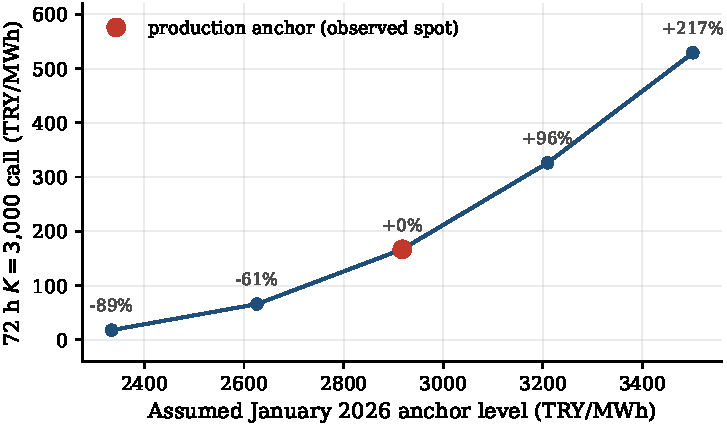
\includegraphics[width=\textwidth]{figures/anchor_sensitivity.pdf}
\caption{Option value against the assumed January anchor level, curve shape
rule held fixed.}
\label{fig:anchorsens}
\end{figure}

\paragraph{Persistence is the dominant residual-layer input.}
The archived specification inherited its mean-reversion rate from an
autoregressive fit to the untransformed price level, giving
$\phi = 0.999996$, $\kappa = 4.11\times10^{-6}$ h$^{-1}$ and a within-regime
half-life near nineteen years. Under that value the same contract prices at
$687.04$ \TRY, more than four times the production figure, because a
near-unit-root residual accumulates variance almost linearly in horizon instead
of saturating. The correction substitutes the deseasonalised single-regime
coefficient $\phi = 0.9246$, giving $\kappa = 0.0784$ h$^{-1}$ and the
saturating dispersion path of Figure~\ref{fig:residualsd}.

The two figures are not in conflict once the objects are separated. A
Markov-switching AR(1) has a marginal autocorrelation that mixes a fast
component, decaying at rate $q_{01}+q_{10}\approx 0.398$ h$^{-1}$, with a slow
component decaying at $-\ln\phi$. Because the regime-conditional means here are
small and close together, the regime-shift contribution to variance is around
$5\%$, so the marginal autocorrelation is dominated by the slow component. A
$200{,}000$-hour simulation confirms an empirical half-life consistent with the
near-unit-root value to within $2\%$ of theory. The nineteen-year figure
correctly describes persistence of the raw transformed price, which over the
estimation window absorbs lira depreciation; it does not describe persistence of
deviations around a forward curve, which is the object \eqref{eq:ou} requires.
Diagnosing this took separating two quantities that a single reported statistic
had conflated.

\paragraph{What the centring buys.}
Running the same parameter set through the archived multiplicative specification
of Remark~\ref{rem:multiplicative}, which lets the residual dynamics determine
the implied forward rather than anchoring it, gives Figure~\ref{fig:legacy}. The
centred form returns $F(T)$ at every horizon. The multiplicative form, on
identical parameters, converges instead to an implied expected spot near
$-3{,}108$ \TRY{} against an observed forward of $+2{,}916$ \TRY. The sign
arises from the regime-weighted mean in transform space rather than from the
variance inflation dominating under the archived mean-reversion rate, so the
specification fails differently at different parameter values while failing in
both. This is the practical content of Proposition~\ref{prop:centering}: forward
consistency is either imposed or it is not obtained.

\begin{figure}[htbp]
\centering
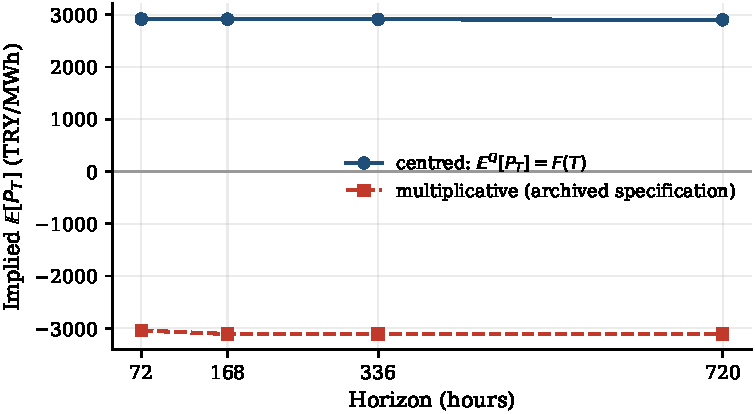
\includegraphics[width=\textwidth]{figures/legacy_vs_centered.pdf}
\caption{Implied expected spot, centred against archived multiplicative
specification.}
\label{fig:legacy}
\end{figure}

\paragraph{The covariate channel is economically signed.}
Shifting the residual demand path by $-2\sigma$ raises the call by $20.4\%$ and
by $+2\sigma$ lowers it by $35.2\%$ (Figure~\ref{fig:rdsweep}), with terminal
dispersion moving from $608$ to $404$ \TRY{} across the same range. The sign
follows from the estimated slopes: $\gamma_{01}<0$ means high residual demand
suppresses transitions into the high-variance regime in this specification.

That direction runs against the intuition that scarcity drives volatility, and
it deserves comment. Two considerations make it less surprising than it first
appears. The regimes here are variance states in transform space rather than
economic stress states, as Appendix~\ref{app:transitions} notes, so the relevant
question is when hourly price variability is large rather than when prices are
high. And low residual demand is precisely the condition under which
renewable output displaces the flexible thermal units that would otherwise
absorb short-run imbalances, leaving a supply stack with less capacity to
respond smoothly. The realised sample is consistent with this reading: across
the seven evaluation months, the correlation between the monthly mean price and
the monthly standard deviation of realised prices is $-0.67$, with the
highest-price month showing the lowest dispersion ($573$ \TRY) and one of the
lowest-price months the highest ($1{,}258$ \TRY). With seven observations this
is suggestive rather than conclusive, and we do not treat it as a test.

The direction is therefore reported as a property of the estimated coefficients,
not as an established economic finding, since the omitted ramp covariate
documented in Section~\ref{sec:provenance} could alter it and the intercepts
entering the same logistic functions are reconstructions rather than estimates.

\begin{figure}[htbp]
\centering
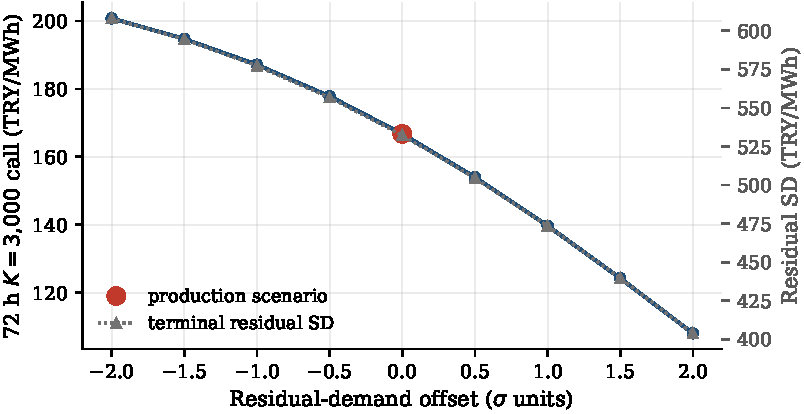
\includegraphics[width=\textwidth]{figures/rd_sweep.pdf}
\caption{Call value and terminal dispersion across a $\pm2\sigma$ range of
residual-demand offsets.}
\label{fig:rdsweep}
\end{figure}

\paragraph{Everything else is second order.}
Substituting the regime volatilities of the closest competing estimated model
changes the price by $0.70\%$, despite a large difference in fit criteria between
the two specifications. The discount rate is similarly immaterial across
$r\in[0.15,0.60]$, a range bracketing Turkish policy rates over the period: at
$720$ hours the factor $e^{-rT}$ moves only from $0.988$ to $0.952$. That is a
property of the maturities studied rather than evidence that the assumption is
innocuous in general, and contracts extending over several months would require
the term structure of rates to be modelled rather than assumed. Initialising the
chain at its stationary distribution rather than the filtered one is likewise
immaterial at $72$ hours, since with mean regime durations under eight hours the
chain has forgotten its initial condition well before expiry; the same
substitution moves a $6$-hour option by roughly $29\%$, so the irrelevance again
belongs to the horizon rather than to the parameter. The drift premium channel is
quadratically suppressed, as established in Section~\ref{sec:q1}.

\subsection{Realised evaluation}
\label{sec:realised}

The forward curve constructed at the end of 2025 can be compared against what
subsequently occurred. Table~\ref{tab:realised} reports, for each delivery month,
the realised mean, the bias of the curve against it, the mean absolute error, the
symmetric percentage error, and a dispersion ratio comparing mean model residual
standard deviation to the realised standard deviation of realised-minus-forward
within that month. Figure~\ref{fig:backtest} plots the two series as daily means together with the
monthly biases, the January bar distinguished because its level comes from the
anchor rather than from a quote.

\begin{table}[htbp]
\centering
\caption{Realised evaluation against the production forward curve, January to
July 2026.}
\label{tab:realised}
\small
\setlength{\tabcolsep}{4.5pt}
\begin{tabular}{@{}lrrrrrr@{}}
\toprule
Month & Hours & Realised mean & Bias & MAE & sMAPE & Disp.\ ratio \\
\midrule
2026-01$^{\dagger}$ & 744 & 2{,}894.92 & $-14.47$ & 451.93 & 16.8\% & 0.97 \\
2026-02 & 672 & 2{,}078.20 & $-822.79$ & 992.40 & 50.0\% & 0.56 \\
2026-03 & 744 & 1{,}620.32 & $-935.99$ & 1{,}193.58 & 71.5\% & 0.46 \\
2026-04 & 720 & 921.06 & $-1{,}579.60$ & 1{,}873.41 & 126.3\% & 0.41 \\
2026-05 & 744 & 590.90 & $-1{,}915.35$ & 2{,}150.69 & 155.2\% & 0.44 \\
2026-06 & 720 & 1{,}240.16 & $-1{,}005.17$ & 1{,}458.19 & 101.3\% & 0.35 \\
2026-07 & 744 & 2{,}699.61 & $-858.58$ & 1{,}058.33 & 40.9\% & 0.61 \\
\midrule
Overall & 5{,}088 & 1{,}721.72 & $-1{,}019$ & 1{,}312.39 & 80.4\% & --- \\
\bottomrule
\end{tabular}

\vspace{2pt}
\footnotesize $^{\dagger}$ January carries no observed quote; its curve level
is the near-term anchor assumption.
\end{table}

\begin{figure}[htbp]
\centering
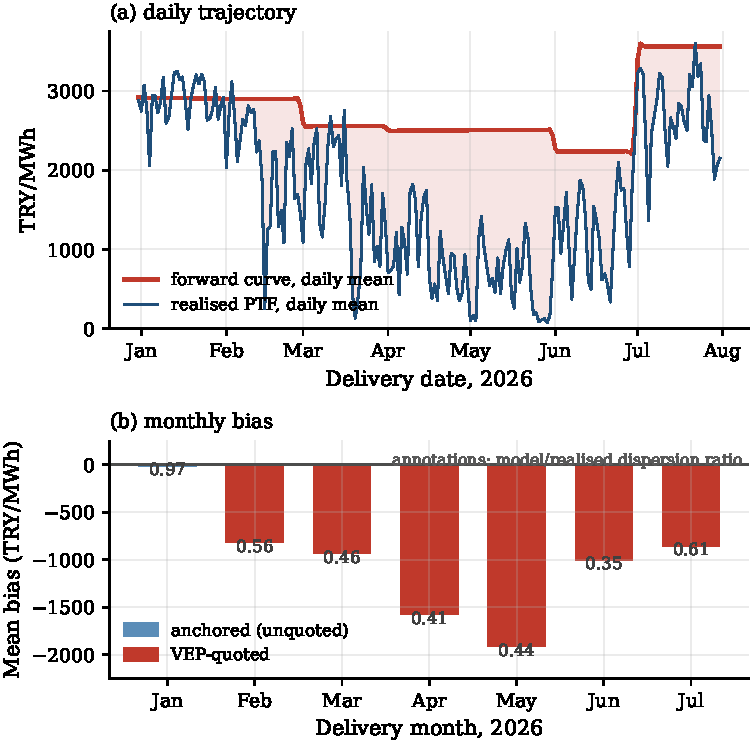
\includegraphics[width=\textwidth]{figures/backtest.pdf}
\caption{Realised evaluation. Panel (a) plots realised PTF against the
production forward curve as daily means; panel (b) gives the monthly mean bias,
with the anchored January window distinguished from the VEP-quoted months.}
\label{fig:backtest}
\end{figure}



Three observations follow, and we state them in order of how much they
constrain the interpretation of the rest of the paper.

First, the forward strip missed badly. Realised prices fell below the quoted
forward in every month from February onwards, by $24\%$ in July and by $76\%$ in
May, with an overall mean bias of $-1{,}019$ \TRY. In May, $222$ of $744$
delivery hours cleared below $10$ \TRY. The magnitude of the deviation is
consistent with a large supply-side shock rather than with ordinary forecast
error, and the period coincided with exceptionally favourable hydrological
conditions and record renewable output that displaced gas-fired generation from
the merit order. We describe the coincidence and do not estimate it; attributing
the deviation causally would require a supply-stack decomposition that we do not
perform, and the merit-order mechanism is well documented elsewhere
\citep{Sensfuss2008,Ketterer2014,Clo2015,SirinYilmaz2020}.

Second, because our curve reproduces the quotes exactly, the entire level error
is inherited from the forward market. No property of the residual
specification, the regime structure or the pricing scheme contributed to it. The
error therefore bounds what forward-anchored valuation can deliver in this
market, and the bound is not a small one: an option value anchored to a forward
curve that is subsequently wrong by $40\%$ on average is wrong by a
correspondingly large amount, however carefully the distribution around the
curve was specified. This is a structural property of the anchoring approach
rather than a defect of our implementation, and it applies equally to any of the
curve-construction methods cited in Section~\ref{sec:curve}.

Third, the month that was not quoted performed best. January, whose level came
entirely from the near-term anchor assumption, shows a bias of $-14.47$ \TRY{}
and the lowest sMAPE in the sample, while every quoted month missed by hundreds
of lira. We caution against reading this as evidence that the anchor rule
outperforms the market. The anchor was set at the observed spot and interpolated
towards February, so it inherited the information content of a price observed
one hour before the window opened, whereas the quoted months encode expectations
formed up to seven months ahead. The comparison illustrates how rapidly forward
information decayed during this episode rather than the merits of an
interpolation rule.

\subsection{Evidence from seven valuation dates}
\label{sec:multidate}

A single valuation date cannot distinguish an unusual episode from a persistent
property of the quote strip. The curve construction can be replayed at earlier
dates without contamination, because it uses only the quotations published on
the valuation date and the spot of that hour and contains no historical
parameter. The residual dynamics cannot be replayed, since their parameters are
fitted to data through 2025, so this exercise evaluates the forward curve alone
and prices no option. Seven valuation dates at six-month intervals from
2022-12-31 to 2025-12-31 yield $49$ (date $\times$ delivery month)
observations. Replaying 2025-12-31 through the same code reproduces the
published curve to $4.5\times10^{-13}$ \TRY{} over $5{,}089$ hours.

Three results follow, and the first revises the reading of
Section~\ref{sec:realised}.

\paragraph{The front month is never quoted.} The anchor rule fires at all seven
dates. Every strip prices delivery months two through seven ahead and none
prices the first, so the structural claim of Section~\ref{sec:anchor} holds
across three years rather than resting on one observation.

\paragraph{2026 is large but not exceptional.} The $-1{,}019$ \TRY{} mean bias
of the 2025-12-31 curve sits at the $32.7$th percentile of the pooled
distribution and the $28.6$th percentile of the seven date means, inside their
interquartile range. Two earlier dates produced more negative outcomes, the
worst being 2022-12-31 at $-1{,}465$ \TRY{} ($-39.8\%$). The hydrological
episode of 2026 is therefore an instance of a magnitude the strip has produced
before, not a departure from otherwise reliable behaviour.

\paragraph{The bias is large, negative on average, and unstable in sign.}
Pooled across dates the mean bias is $-603$ \TRY{} ($-18.2\%$ in relative terms)
with a standard deviation of $775$ \TRY. Realised prices came in below the strip
at five dates and above it at two, with date means running from $-1{,}465$ to
$+290$ \TRY{} (Figure~\ref{fig:multidate}a). The direction is not a stable
property. Statistical support for a non-zero mean is correspondingly weak once
dependence is respected: pooling all $49$ observations gives $t=-5.45$, but the
same delivery month appears from several valuation dates and consecutive months
of one curve share a market state, so that figure is anti-conservative.
Aggregating to one observation per date gives $t=-2.29$ on seven dates,
$p=0.062$, and restricting to non-overlapping delivery windows leaves $p$
between $0.11$ and $0.49$. We therefore report the mean bias as economically
large and describe the strip as a biased and unstable predictor, without
claiming a calibrated significance level on seven dates.

\begin{table}[htbp]
\centering
\caption{Mean bias of the forward curve against realised monthly baseload, by
valuation date. Seven delivery months per date.}
\label{tab:multidate}
\small
\setlength{\tabcolsep}{6pt}
\begin{tabular}{@{}lrrr@{}}
\toprule
Valuation date & Mean bias (\TRY) & Median (\TRY) & Relative (\%) \\
\midrule
2022-12-31 & $-1{,}464.63$ & $-1{,}545.59$ & $-39.8$ \\
2023-06-30 & $-1{,}250.01$ & $-1{,}299.88$ & $-36.5$ \\
2023-12-31 & $-756.89$    & $-813.27$     & $-24.5$ \\
2024-06-30 & $-174.47$    & $-214.48$     & $-6.2$ \\
2024-12-31 & $+151.28$    & $+179.60$     & $+7.2$ \\
2025-06-30 & $+289.76$    & $+307.18$     & $+11.4$ \\
2025-12-31 & $-1{,}018.85$ & $-935.99$    & $-39.1$ \\
\midrule
Pooled ($n=49$) & $-603.40$ & $-353.70$ & $-18.2$ \\
\bottomrule
\end{tabular}
\end{table}

\begin{figure}[htbp]
\centering
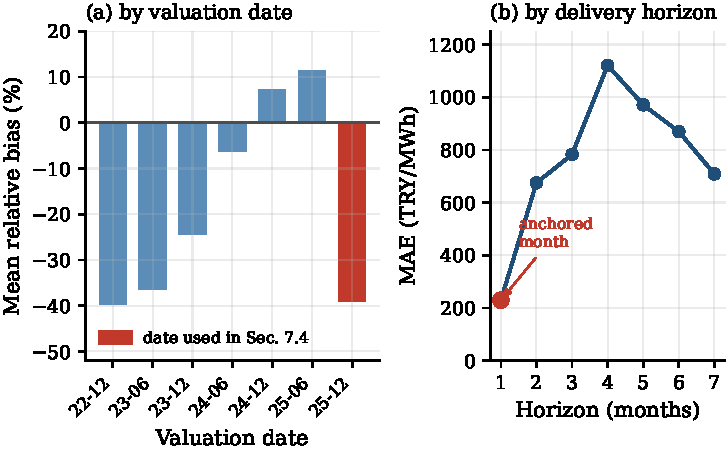
\includegraphics[width=\textwidth]{figures/multi_date.pdf}
\caption{Forward curve error across seven valuation dates. Panel (a) gives the
mean relative bias per date; panel (b) the mean absolute error by delivery
horizon.}
\label{fig:multidate}
\end{figure}

\paragraph{The anchor band has approximately the right scale.} The $\pm20\%$
band used in Section~\ref{sec:anchorsens} was chosen without empirical support.
Across the seven anchored months the realised relative error has a standard
deviation of $11.7\%$, against $11.5\%$ for a uniform distribution on
$\pm20\%$, so the band is of the right width. It is not a containment bound:
one of seven anchored months falls outside it, at $-21.2\%$. And its centre is
displaced, the empirical mean being $-3.5\%$, so the linear ramp over-prices the
anchored month slightly on average. The band should be read as a scale for
anchor uncertainty rather than as a range that brackets it.

\paragraph{Error does not grow monotonically with horizon.}
Figure~\ref{fig:multidate}b shows mean absolute error rising from $229$ \TRY{}
at the anchored first month to $1{,}121$ \TRY{} four months ahead, then falling
back to $708$ \TRY{} at seven, with a Spearman rank correlation of $+0.25$
between horizon and absolute error. The decline at the long end should not be
read as skill. The first horizon is always the anchored month, so its small
error reflects a ramp from an observed spot rather than a quoted forward, and
with dates six months apart the seventh horizon is always the same pair of
calendar months, making the long end as much seasonal as maturity-driven.

Four of the seven valuation dates fall on a non-business day, when no index
price is published; for those the strip is the last publication before the date,
one to four days stale, while the spot remains that of the valuation night. No
later publication is used anywhere, the affected observations are flagged in the
released data rather than dropped, and a strict same-day rule would reduce the
study to three dates.

A fourth observation concerns the model's own dispersion. The ratio of model
residual standard deviation to realised dispersion is $0.97$ in January and
falls to $0.35$--$0.61$ thereafter, so outside the anchored window the model is
too narrow by a factor of roughly two. Part of this is expected: the production
residual is a single-factor approximation, and a companion two-factor
specification developed alongside this work carries an additional slow component
that the production configuration does not represent. Part is the shock itself,
which widened realised dispersion beyond anything the historical sample
contains. We do not attempt to separate the two here.
